\documentclass[conference]{IEEEtran}

\usepackage{amsmath}
\usepackage{algorithmic}
\usepackage{graphicx}
\usepackage{textcomp}
\usepackage{xcolor}
\def\BibTeX{{\rm B\kern-.05em{\sc i\kern-.025em b}\kern-.08em
    T\kern-.1667em\lower.7ex\hbox{E}\kern-.125emX}}

% setup BibTex
\usepackage[
backend=biber,
style=ieee,
url=false,
isbn=false,
eprint=false
]{biblatex}
\addbibresource{references.bib}

% utility 
\usepackage{booktabs} % better tables
\usepackage{subcaption}
\usepackage{microtype}
\usepackage{comment}
\usepackage{siunitx}
\usepackage{lipsum}

% circuitikz
\usepackage[straightvoltages, american, europeanresistors, cuteinductors, RPvoltages]{circuitikz}

% cleverref, must be last
\usepackage[capitalise]{cleveref}

\begin{document}

\title{Influence of Encapsulation on Core Loss of Ferrites in Inductive Power Transfer}

\author{
  Alexander K. Bailey, Jerry Sun\textsuperscript{\textdagger}, Seho Kim, Willsen Wijaya\textsuperscript{\textdagger}, Tom Allen\textsuperscript{\textdagger}, Grant A. Covic\\
  \textit{Department of Electrical, Computer and Software Engineering}\\
  \textit{\textsuperscript{\textdagger}Centre for Advanced Materials Manufacturing and Design}\\
  \textit{University of Auckland}\\
  Auckland, New Zealand\\
  \{alexander.bailey, jerry.sun, seho.kim, willsen.wijaya, tom.allen, ga.covic\}@auckland.ac.nz\\ 
}
\maketitle
\thispagestyle{plain}
\pagestyle{plain}

\begin{abstract}
  Inductive power transfer (IPT) magnetics are often `potted' with an encapsulant material to improve thermal performance.
  The curing process of common thermoset encapsulant materials creates a mechanical load which permanently reduces the magnetic performance of the core material. 
  This article measures how the core loss of Mn--Zn ferrites changes with an applied compressive stress of \textcolor{red}{\SIrange{10}{100}{\mega\pascal}} at \SI{85}{\kilo\hertz}. 
  At maximum load, the core loss increases by 
  The measured data informs a multi-physics simulation model which predicts the increase in losses in a practical potted IPT pad with \textcolor{red}{\SI{10}{\percent}} error, demonstrating a \textcolor{red}{\SI{140}{\percent}} increase in core loss. 
\end{abstract}

\begin{IEEEkeywords}
Core loss, inductive power transfer (IPT), loss measurement, magnetic losses
\end{IEEEkeywords}

\section{Introduction}

\IEEEPARstart{E}{lectric} vehicles (EVs) are increasingly common due to lowering costs and a rising need for climate change. 
However, existing infrastructure favours the outgoing Internal Combustion Engine Vehicles (ICEVs), meaning charging EVs can be cumbersome. 
Inductive power transfer (IPT) is a wireless charging technology that enables power transfer using magnetic fields. 
The application of this technology to the charging of EVs could enable more reliable and convenient charging of EVs of all power levels \cite{covicModernTrendsInductive2013b}. 

At higher power levels, thermal issues limit power density. 
In order to improve the thermal performance of the IPT magnetics, both the coil and core layer (shown in \cref{fig:padstructure}) are `potted' in an encapsulant material \cite{kneidlProcessingInfluencesResinbased2020}. 
Typical encapsulant materials have high thermal conductivity which improves the temperature profile uniformity and allows for a higher current density in the coil. 
However, several articles have noted the deterimental effect of encapsulant materials on the magnetic performance of ferrites. 

Polycrystalline ferrites show decreased magnetic permeability and a widening $B$-$H$ curve under applied pressure due to the compressed topography of the domain walls \cite{leflochEffectPressureSoft1981}. 
Foote et. al verified the reduction in permeability and increased core loss through the construction of a small-scale potted IPT coil assembly, demonstrating a \SI{\sim 100}{\percent} increase in losses \cite{footeEncapsulationResidualStress2023}.
This article aims to measure the effect of pressure on ferrite core loss at \SI{85}{\kilo\hertz} in a geometry independent and reproducable manner with standard core loss measurement techniques. Such that designers can better predict the impacts of encapsulation on the IPT system's behaviour. 

\begin{figure}[t]
  \centering
  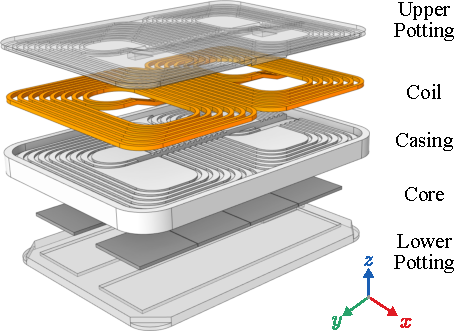
\includegraphics{figures/padstructure.pdf}
  \caption{Typical structure of IPT pad for EV charging}
  \label{fig:padstructure}
\end{figure}

\section{Characterisation of Ferrite Under Load}

\subsection{Methodology}

\cref{fig:compressionholder} shows an overview of the designed setup. 

\begin{figure}
  \centering
  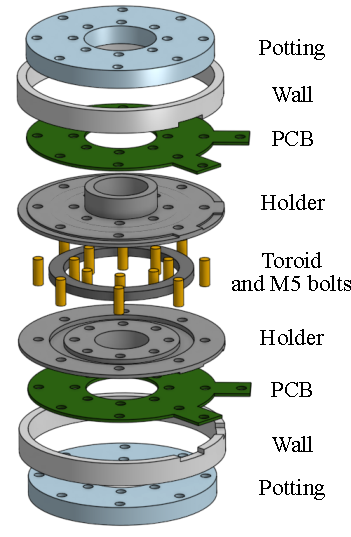
\includegraphics{figures/compressionholder.pdf}
  \caption{Exploded diagram of designed toroid compression setup}
  \label{fig:compressionholder}
\end{figure}

\begin{table}
  \centering
  \caption{Toroid properties}
  \begin{tabular}{@{}llll@{}}
    \toprule
    Parameter & Value & Parameter & Value \\ \midrule
    Material & TDK N95 & $L_\text{p}$ & \textcolor{red}{\SI{5}{\micro\henry}} \\
    Inner Diameter & \SI{64}{\milli\meter} & $L_\text{s}$ & \textcolor{red}{\SI{5}{\micro\henry}} \\
    Outer Diameter & \SI{80}{\milli\meter} & $k$ & \textcolor{red}{$0.99$} \\
    $N_\text{p}$ & 4 & $R_\text{w,p}$ & \textcolor{red}{\SI{119}{\milli\ohm}} \\
    $N_\text{s}$ & 4 & $R_\text{w,s}$ & \textcolor{red}{\SI{119}{\milli\ohm}} \\
    \bottomrule
  \end{tabular}
  \label{tab:toroidproperties}
\end{table}
\begin{figure*}[t]
  \centering
  \begin{subfigure}{\columnwidth}
    \centering
    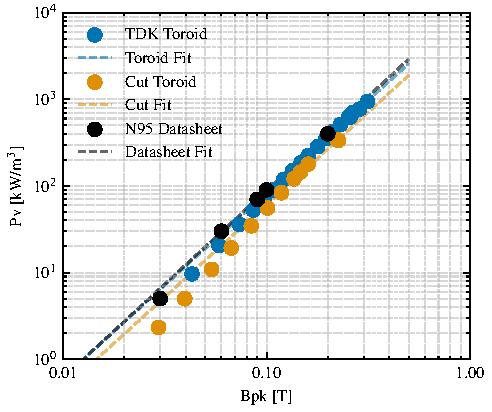
\includegraphics{figures/24-09-10_BP_curves.pdf}
    \caption{}
    \label{fig:BPcurves}
  \end{subfigure}~
  \begin{subfigure}{\columnwidth}
    \centering
    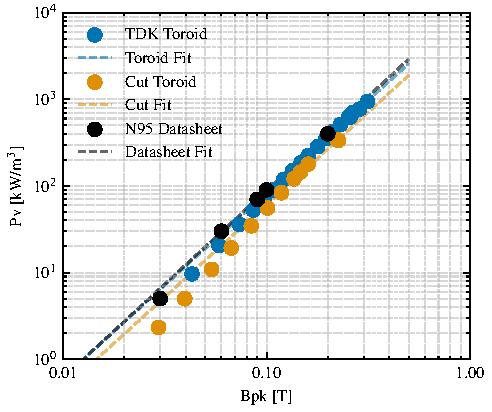
\includegraphics{figures/24-09-10_BP_curves.pdf}
    \caption{}
    \label{fig:corelossstress}
  \end{subfigure}

  \begin{subfigure}{\columnwidth}
    \centering
    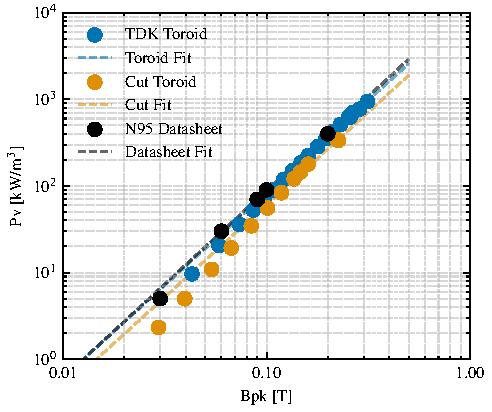
\includegraphics{figures/24-09-10_BP_curves.pdf}
    \caption{}
    \label{fig:BPcurves}
  \end{subfigure}~
  \begin{subfigure}{\columnwidth}
    \centering
    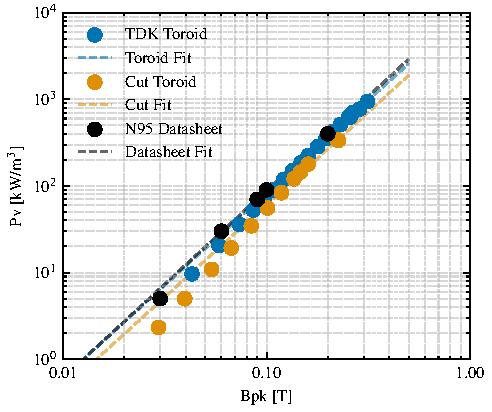
\includegraphics{figures/24-09-10_BP_curves.pdf}
    \caption{}
    \label{fig:corelossstress}
  \end{subfigure}
  \caption{(a) $B$-$P$ curves of the TDK N95 ferrite toroid under several levels of compressive loading $\overline{\sigma_\text{eqv}}$, (b) Core loss of TDK N95 ferrite toroid under several levels of compressive loading at \SI{\sim 5}{\milli\tesla}, \SI{\sim 25}{\milli\tesla}, \SI{\sim 50}{\milli\tesla} and \SI{\sim 100}{\milli\tesla}, \SI{85}{\kilo\hertz}, (c) Reduction in permeability after loading is removed, (d) Increasing core loss after loading is removed}
\end{figure*}

Toroids of TDK N95 ferrite were cut from \SI{5}{\milli\meter} tiles using a water jet cutter and wound with litz on the primary and magnet wire on the secondary. 
The toroid properties are given in \cref{tab:toroidproperties}.
The machining of ferrite has also been shown to increase core losses due to the mechanical stress imposed on the surface during the cutting process \cite{neumayrOriginQuantificationIncreased2019}. 
However, this effect is concentrated on the cut surface which for this case is the outer and inner surfaces, not in the mean flux path of the toroid hence the effects are expected to be minimal. 
Regardless, the following experiments include a factory-epoxy-coated R34 toroid of TDK N95 ferrite as a reference. 

For each mechanical loading scenario, the core loss $P_\text{core}$ was then measured using a partial cancellation method which modifies the conventional two-winding core loss measurement method with a compensation capacitor $C_s$ in series to cancel the reactive voltage across the inductor under test $L_t$ \cite{houNewHighFrequencyCore2017}. 
The equivalent circuit of this method is shown in \cref{fig:partialcancellationcircuit}.
$C_s$ could be selected to completely cancel the reactive power in the system, but maintaining resonance for different operating conditions is challenging. 
Instead, a partial cancellation method defines a voltage cancellation factor $k_v$, the ratio of the cancelled reactive voltage to the total reactive voltage, to only `partially' cancel the reactive component of $L_t$. 
In order to determine the value of $k_v$, a phase pertubation is introduced into $i_L$, creating \cref{eqn:pcoreprime}, $k_v$ can then be calculated by combining \cref{eqn:pcore} and \cref{eqn:pcoreprime}.
Using this method core loss was calculated from measurements of the current flowing through the primary winding $i_L(t)$, the voltage on the secondary winding $v_2(t)$ and the voltage across the compensation capacitor $v_C(t)$ by, 
\begin{equation}
  P_\text{core} = f \int_0^T v_2(t)i_L(t)dt + \frac{f}{k_v} \int_0^T v_c(t)i_L(t) dt
  \label{eqn:pcore}
\end{equation}
\begin{equation}
  P_\text{core}^{\prime} = f \int_0^T v_2(t)i_L^{\prime} (t)dt + \frac{f}{k_v} \int_0^T v_c(t)i_L^{\prime}(t) dt
  \label{eqn:pcoreprime}
\end{equation}
\begin{equation}
  k_v = \frac{\int_0^T v_c(t)i_L(t)dt - \int_0^T v_ci_L^\prime(t)dt}{\int_0^T v_2(t) i_L^\prime(t) dt - \int_0^T v_2(t) i_L(t) dt}
  \label{eqn:kv}
\end{equation}

\begin{figure}[t]
  \begin{subfigure}{\columnwidth}
    \centering
    \begin{circuitikz}
    \ctikzset{quadpoles style=inline}

    % Voltage source
    \draw (0,-3) to[sV, l=$V_\text{pa}$] (0,2);

    % I_L
    \draw (0,2) to[short, i^=$i_\text{L}(t)$] (1,2);

    % Winding resistance 
    \draw (1,2) to[R, R=$R_{w}$] (3,2);

    % Transformer
    \draw (6,2) node[transformer core, anchor=A1] (T) {}
      (T.A1) -- ++(-1.5,0) coordinate(TPa)
      (T.A2) to[short] ++(-1.5,0) coordinate(MDa);

    \draw (TPa) to[L, L=$L_\text{m}$] (MDa);
    \draw (TPa) to[short] ++(-1.5,0) coordinate(TP);
    \draw (MDa) to[short] ++(-1.5,0) coordinate(MD);
    \draw (TP) to[R=$R_\text{core}$] (MD);

    \draw (T.B1) -- ++(.5, 0) coordinate(TPb)
    to[open, v^<=$$, o-o] (TPb |- T.B2)
    -- (T.B2);

    % manually add v2 label
    \node[right] at (TPb -| T.B1) [xshift=0.5cm, yshift=-1.1cm] {$v_2(t)$};

  % Turns ratio label
    \node at ($(T.A1)!0.5!(T.B1)$) [above=0cm] {$N_p : N_s$};

    % Capacitor
    \draw (MD) to[C, a=$C_\text{s}$, v^=$v_C(t)$] (3,-3);

    \draw (3,-3) -- (0,-3);

    % Dashed box around Rw, Rcore, Lm, and transformer
    \draw[dashed] (1, 3) rectangle (8.3, -.5)
    node[above, midway, yshift=2cm, font=\itshape] {Wound toroid};

\end{circuitikz}

    \caption{}
    \label{fig:partialcancellationcircuit}
  \end{subfigure}

  \vspace{1em}

  \begin{subfigure}{\columnwidth}
    \centering
    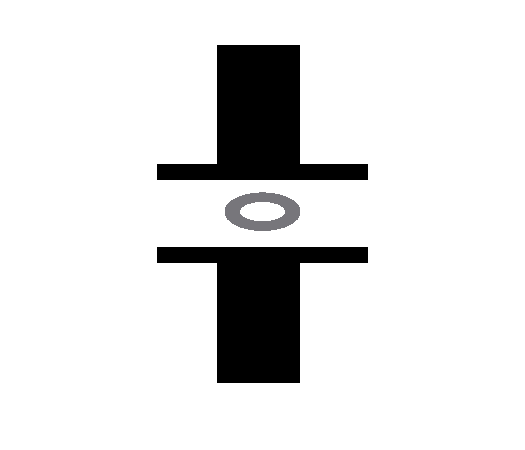
\includegraphics{figures/experimentalsetup.pdf}
    \caption{}
    \label{fig:experimentalsetup}
  \end{subfigure}
  \caption{(a) Equivalent circuit of the partial cancellation method, (b) Experimental setup for core loss measurement under compressive stress}
\end{figure}
\subsection{Loaded Toroid Results}

\cref{fig:BPcurves} shows the measured $B$-$P$ curve for each of the loading scenarios of the cut toroid and a reference manufacturer provided toroid. 
The unloaded cut toroid has slightly lower loss density than the manufacturer epoxied toroid, despite the stress-state from machining. 
This shows that the machined toroid is suitable for these measurements. 

The stress-dependent behaviour of ferrite has been shown to have a memory effect. 
After the compressive loading is removed, the permeability of the material is decreased and the core loss increases. 
In order to account for this, each sample is measured before, during and after loading. 
The results presented in \cref{fig:BPcurves} and \cref{fig:corelossstress} are all under active loading, while \cref{fig:reductionpermeability} shows the change in relative permeability $\mu_r$ after the loading is removed compared to before the first loading scenario. 

\lipsum[1]

\section{Multiphysics Modelling of Potted IPT Pad}
\label{sec:modelling}

Ferrite losses are non-linearly related to temperature and, as shown previously, compressive stress. 
Due to the thermal expansion of the constituent materials, both the thermal and mechanical physics are heavily coupled, this expansion creates compressive stresses which effect the electromagnetic (EM) simulation. 
In order to predict the core loss of potted IPT pads operating at a thermal steady-state, this article proposes a multiphysics simulation methodology presented in \cref{fig:simulationflowchart}. 
All FEA simulations are conducting using Ansys Workbench, Ansys Maxwell for EM results, Ansys Mechanical for the stress-strain results and Ansys Steady-state Thermal for temperature predition. 

\begin{figure}[t]
  \centering
  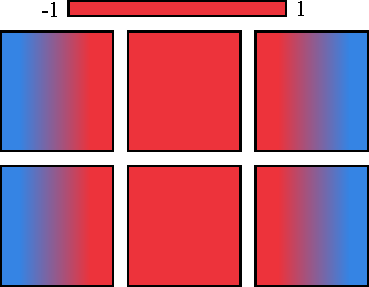
\includegraphics{figures/simulatedpottingpadstresses.pdf}
  \caption{FEA simulation of ambient residual stress due to cure shrinkage on ferrite tiles at \SI{25}{\celsius} after curing}
  \label{fig:pottingstresses}
\end{figure}

The residual stresses are calculated by structural FEA simulation assuming a constant body temperature of $T_\text{cure}$ cooling to ambient (\SI{25}{\celsius}). 
The cure shrinkage is accounted for by modelling a displacement of the potting material based on the manufacturer stated cure shrinkage, i.e. for cure shrinkage of \SI{1}{\percent} a fixed deformation is applied to each face such that the total volume of the body reduces by \SI{1}{\percent}.
The results of this simulation are shown in \cref{fig:pottingstresses}. 
This simulation models only the ferrites, casing and lower potting region shown in \cref{fig:padstructure} since the designed magnetics separates the casing in to two cavities and the Litz wire was shown to have minimal effect on the residual stresses in preliminary simulations. 
The obtained residual stress-strain distribution is then used as an initial condition for the operational stress-strain simulation which models the full pad. 

The simulations are set up for the designed \textcolor{red}{\SI{30}{\kilo\volt\ampere}} with only a single pad to reduce modelling complexity. 
This approximates the excitation required for an IPT system transferring \SI{11}{\kilo\watt}. 
The addition of a second pad should not affect the results of these simulations assuming that the airgap is large enough to prevent thermal interaction between the two sets of magnetics, which is typical for EV charging applications.

\begin{figure}
  \usetikzlibrary{shapes.geometric, arrows}

\tikzstyle{process} = [rectangle, rounded corners, minimum width=3cm, minimum height=1cm, text centered, draw=black, fill=orange!30]
\tikzstyle{arrow} = [thick,->,>=stealth]

\begin{tikzpicture}[node distance=2cm]

% Nodes
\node (start) [process] {Start Simulation};
\node (electrical) [process, below of=start] {Electrical Model};
\node (thermal) [process, below of=electrical] {Thermal Model};
\node (mechanical) [process, below of=electrical, yshift=-2cm] {Mechanical Model};
\node (convergence) [process, below of=mechanical] {Convergence Check};
\node (stop) [process, below of=convergence] {Stop Simulation};

% Arrows
\draw [arrow] (start) -- (electrical);
\draw [arrow] (electrical) -- (thermal) node[midway,left] {$P_\text{litz}$, $P_\text{core}$};
\draw [arrow] (thermal) -- (mechanical) node[midway,left] {$\Delta T$};
\draw [arrow] (mechanical) -- (convergence) node[midway,left] {$\sigma_\text{eqv}$};
\draw [arrow] (convergence) -- (stop);
\draw [arrow] (mechanical.west) -| ++(-1,0) node[midway,above] {$\sigma_\text{res}$} -- (mechanical.west);
\draw [arrow] (mechanical.east) -- ++(1.5,0) |- (electrical.east) node[midway,above] {$P_\text{core}\left(T_\text{core}, \overline{\sigma_\text{eqv}}\right)$};
\draw [arrow] (thermal.east) -- ++(1.5,0) |- (electrical.east) node[midway,right] {};
\draw [arrow] (convergence.east) -- ++(3,0) |- (start.east) node[midway,right] {};

\end{tikzpicture}

  \caption{Flowchart of the multiphysics simulation including residual stress initial conditions and induced thermal stresses during operation}
  \label{fig:simulationflowchart}
\end{figure}

\subsection{Electromagnetic Domain}

\lipsum[2]

\subsection{Structural Domain} 

\lipsum[2]

\begin{table}
  \centering
  \caption{Mechanical properties of relevant materials}
  \begin{tabular}{@{}llll@{}}
    \toprule
    Material & Manufacturer & $\alpha$ $\times 10^{-6}$ & $Y$ \\ \midrule
    N95 Ferrite & TDK & $10$ & \SI{119}{\giga\pascal} \\
    5083 Aluminium & TDK & $10$ & \SI{119}{\giga\pascal} \\
    UR5608 & TDK & $10$ & \SI{119}{\giga\pascal} \\
    PX900D & TDK & $10$ & \SI{119}{\giga\pascal} \\
    ER2223 & TDK & $10$ & \SI{119}{\giga\pascal} \\
    \bottomrule
  \end{tabular}
\end{table}

\subsection{Thermal Domain}

\lipsum[2]

\section{Experimental Verification}

This section describes the construction and validation of an \SI{11}{\kilo\watt} DD IPT coil structure potted with UR5608 polyurethane encapsulation material. 
The pad is measured under initial (ambient temperature) conditions before and after potting. 
The potted pad is then evaluated at steady-state temperature conditions. 
These experiments validate the simulation procedure described in \cref{sec:modelling}. 

\subsection{Pad Construction}

\lipsum[2]

\begin{figure}
  \centering
  \begin{subfigure}{\columnwidth}
    \centering
    \includegraphics[width=3in]{figures/coilside.pdf}
    \caption{}
  \end{subfigure}
  \vspace{1em}

  \begin{subfigure}{\columnwidth}
    \centering
    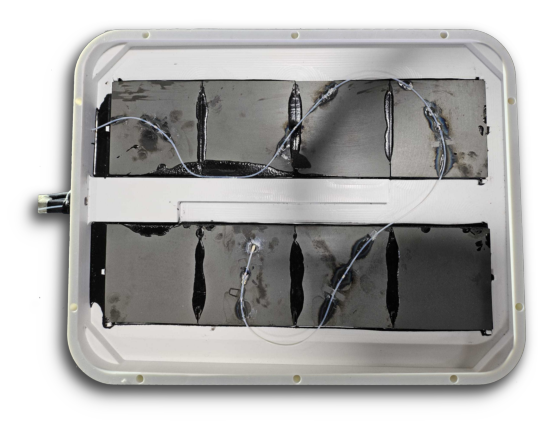
\includegraphics[width=3in]{figures/ferriteside.pdf}
    \caption{}
  \end{subfigure}
  \vspace{1em}

  \begin{subfigure}{\columnwidth}
    \centering
    \includegraphics[width=3in]{example-image-c}
    \caption{}
  \end{subfigure}

  \caption{Construction of IPT pad, (a) unpotted coil layer, (b) unpotted ferrite layer, (c) milled bottom surface of potted pad}
\end{figure}

\subsection{Core Loss Measurements}

The core loss of a Double D IPT pad designed for \textcolor{red}{\SI{11}{\kilo\watt}} was measured using the stepped resonance method described in \cite{kalraPowerLossMeasurement2020}.
At rated current, the unpotted pad showed a total loss of \textcolor{red}{\SI{0}{\watt}}, with \textcolor{red}{\SI{0}{\watt}} of core loss.
When potted in two pours with UR5608, the total loss increased to \textcolor{red}{\SI{0}{\watt}} with \textcolor{red}{\SI{0}{\watt}} of core loss. 
The FEA simulation predicted a core loss of \textcolor{red}{\SI{0}{\watt}}, an error of \textcolor{red}{\SI{0}{\percent}}. 

\lipsum[1]

\begin{figure}[t]
  \centering
\begin{circuitikz}
\draw
    % Voltage source at the top
    (0,0) to[vsourcesin, l=$V_\text{pa}$] (0,4)
    
    % Capacitor in parallel with the voltage source
    (0,4) -- (1.5,4) to[C, l_=$C$] (1.5,2.5) to[R, l_=$r_\text{C}$] (1.5,0) -- (0,0)
    
    % Horizontal inductor forming the start of the L-shape
    (1.5,4) to[L, l=$L$] (4,4)
    
    % Vertical resistors completing the L-shape
    to[R, l=$r_\text{Cu}$] (4,2.66)
    to[R, l=$r_\text{Fe}$] (4,1.33)
    to[R, l=$r_\text{Al}$] (4,0) -- (1.5,0);

    % box around pad 
    \draw[dashed] (2, 5) rectangle (5, -.5)
    node[above, xshift=-.9cm, yshift=4.9cm, font=\itshape] {IPT Pad};

\end{circuitikz}

  \caption{Circuit diagram of SRE method with ESR model for IPT pad including winding, ferrite and aluminium losses}
  \label{fig:sremethodcircuitdiagram}
\end{figure}

\begin{figure}[t]
  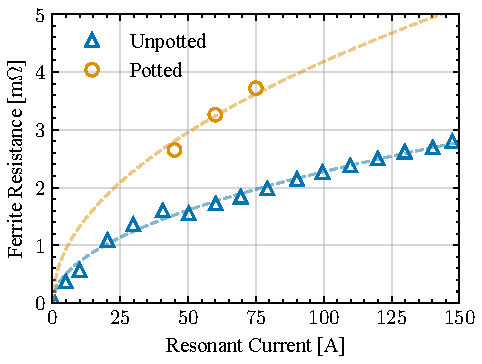
\includegraphics{figures/24-10-17_initialFerriteResistanceComparisonV2.pdf}
  \caption{Measured ferrite resistance against resonant current for the constructed pad before and after potting}
  \label{fig:initialFerriteResistanceComparison}
\end{figure}

\subsection{Thermal Measurements}

\lipsum[2]

\begin{figure}[t]
  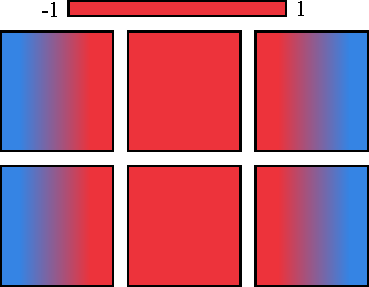
\includegraphics[width=3.5in, height=2in]{figures/simulatedpottingpadstresses.pdf}
  \caption{Predicted steady-state temperature distribution in DD pad under \textcolor{red}{\SI{30}{\kilo\volt\ampere}} operation considering thermal and structural impacts on the ferrites}
  \label{fig:temperaturecomparison}
\end{figure}

\section{Conclusion}

This article has measured the effects of compressive stress on TDK N95 ferrite and applied the gained insight to the multiphysics simulation of an Inductive Power Transfer (IPT) pad. 
Under a \textcolor{red}{\SI{100}{\mega\pascal}} load, the core loss of the N95 ferrite increased by \textcolor{red}{\SI{100}{\percent}}. 
The loading due to residual stresses from the encapsulation process and heating during operation is investigated and the impact is significant. 
Finally, a practical potted DD pad shows a \textcolor{red}{\SI{100}{\percent}} increase in core loss after encapsulation in a polyurethane material. 
Multiphysics simulations which include the mechanical-thermal impacts of the encapsulation material on the magnetic losses matched the temperatures of the DD pad within \textcolor{red}{\SI{20}{\percent}}. 
These results show that the choice of encapsulation material has a significant impact on the thermal and structural behaviour of the IPT pad. 
Designers must trade off electrical, thermal and structural performance to choose a material suitable for the desired application.

\section*{References}
\printbibliography[heading=none]

\end{document}
